\documentclass[12pt]{beamer}
\usetheme{default}
\usefonttheme{serif}

\usepackage{attrib}

\usepackage[backend=biber, citestyle=authoryear]{biblatex}
\addbibresource{references.bib}

\usepackage{graphicx}

\author{Michael Walker}
\title{Runtime Verification}
\institute{Department of Computer Science\\
  University of York\\
  \texttt{msw504@york.ac.uk}
}

\begin{document}

\begin{frame}[plain]
  \titlepage
\end{frame}

%%%%% 1 Minute (1)

\begin{frame}{Outline}
  \tableofcontents

  \begin{center}
    See the handout for literature references.
  \end{center}
\end{frame}

%%%%% 5 Minutes (6)

\section{Static Analysis}
\label{sec:statann}

\begin{frame}{Static Analysis}
  % Very quick overview, cover formal specification, proof assistants,
  % proof-carrying code, and certifying compilers. Get a quite saying
  % it's hard.

  \textbf{Static Analysis:} The (fully or partially) automatic process
  of proving properties of programs prior to executing them.

  \visible<2->{
    \begin{itemize}
      \item Type checking
      \item Memory safety
      \item Deadlock/livelock freedom
      \item Schedulability
    \end{itemize}
  }
\end{frame}

\begin{frame}{Static Analysis: \small A Nemesis Arises!}
  % PAPERS: rice (corollary b)

  \only<1>{
    \begin{quote}
      If $\mathcal P$ is any property possessed by some, but not all,
      recursively enumerable sets, then there exists no effective
      general method for deciding, given a set $\alpha$ by means of a
      partial recursive function enumerating it, whether or not
      $\alpha$ has the property $\mathcal P$.  [\ldots] Of course,
      there will exist special methods for particular functions.

      \attrib{Rice's Theorem, Corollary B, 1953}
    \end{quote}

    There exists no algorithm which can, for all input programs,
    either prove or disprove some nontrivial property $\mathcal P$.
  }

  \visible<2->{
    Suppose we had a function \texttt{identity?} :: $(a \rightarrow a)
    \rightarrow Bool$, which returns ``yes'' or ``no'' depending on
    whether its argument is the identity function.

    \vspace{0.25cm}
  }

  \visible<3->{
    Or even \texttt{identity?} :: $(Bool \rightarrow Bool) \rightarrow
    Bool$

    \vspace{0.25cm}
  }

  \visible<4->{
    We can use this to solve the halting problem!
  }

  \visible<5->{
    \begin{center}
      \texttt{halts?(P, I) = identity?($\lambda$x $\mapsto$ P(I); return x)}
    \end{center}

    Undecidable in general!
  }
\end{frame}

\begin{frame}{Static Analysis: \small Defeating Rice, the Evil Sorcerer}
  Rice's theorem:
  \begin{itemize}
    \item applies to Turing machines,
    \item refers to exact results,
    \item refers to a fully automatic analysis.
  \end{itemize}

  \visible<2->{
    We can:
    \begin{itemize}
      \item weaken our systems,
      \item use heuristics,
      \item introduce human involvement.
    \end{itemize}
  }
\end{frame}

%%%%% 15 Minutes (21)

\section{Runtime Verification}
\label{sec:runver}

\begin{frame}{Runtime Verification}
  % Overview of RV, quote preface of rv'01 proc.

  % "The ultimate longer term goal is to investigate whether the use
  % of lightweight formal methods applied during the execution of
  % programs is a viable component to the current heavyweight methods
  % proving programs correct always before their execution" - RV'01

  % NON-PAPERS: rv01
\end{frame}

%%%%%%%%%% 7 Minutes (13)

\subsection{Design by Contract}
\label{sec:runver-dbc}

\begin{frame}{Design by Contract}
  % Overview of DbC

  % PAPERS: eiffel
\end{frame}

\subsubsection{Annotation Techniques}
\label{sec:runver-dbc-ann}

\begin{frame}{Design by Contract: Annotation Techniques}
  % Talk mostly about JML for source-level, compare and contract
  % BCSL/BML for bytecode-level

  % PAPERS: bcsl, bml
  % NON-PAPERS: jml
\end{frame}

\begin{frame}{Design by Contract: Annotation Techniques}
  % Example contract, talk through
\end{frame}

\subsubsection{Aspect-Oriented Programming Techniques}
\label{sec:runver-sbc-aop}

\begin{frame}{Design by Contract: AOP Techniques}
  % Briefly explain AOP (maybe find a seminal paper?), say this can be
  % used with annotation techniques (eg, AspectJML), but here I'm
  % focusing on writing contracts in the host language and then
  % combining the program logic with the contract checking with
  % AOP. Explain and compare jContractor and ezContract.

  % PAPERS: jcontractor, ezcontract
\end{frame}

%%%%%%%%%% 7 Minutes (20)

\subsection{Trace Analysis}
\label{sec:runver-trace}

\begin{frame}{Trace Analysis}
  % Overview of traces, quote seminal paper (Hoare?), explain how we
  % can generate traces by triggering events at program points
  % (find good paper), and how we can specify properties of programs
  % as properties of traces.

  % PAPERS: cspthy
\end{frame}

\subsubsection{Logics}
\label{sec:runver-trace-log}

\begin{frame}{Trace Analysis: Logics}
  % Overview of regular properties and LTL, find seminal papers using
  % those for RV. Example LTL predicate, explain.

  % PAPERS: eres, alto
\end{frame}

\subsubsection{Monitor-Oriented Programming}
\label{sec:runver-trace-mop}

\begin{frame}{Trace Analysis: Monitor-Oriented Programming}
  % Explain MOP, cite MOP/JavaMOP papers.

  % PAPERS: javamop
\end{frame}

%%%%%%%%%% 1 Minutes (21)

\subsection{Trace Analysis by Contract?}
\label{sec:runver-tbc}

\begin{frame}{Trace Analysis by Contract?}
  % Mention how abstract data types & ghost/model fields in JML/BML
  % let us treat traces, at specification time, as a sequence of
  % events, and reason about that.
\end{frame}

%%%%% 4 Minutes (25)

\section{Conclusions \& Other Work}
\label{sec:conc}

\begin{frame}
  \begin{center}
    \Large Nearly there\ldots
  \end{center}
\end{frame}

\subsection{Runtime Verification has High Overheads}
\label{sec:conc-over}

\begin{frame}{High Overheads}
  % PAPERS: compensate (time)

  Runtime monitoring inevitably leads to time and space overheads.

  \visible<2->{
    \vspace{0.25cm}

    There is work in addressing this:

    \begin{description}
      \item[Space] Analyse the monitoring predicates and simplify,
        % TODO: citation

      \item[Time] Asynchronous monitoring with the ability to roll
        back incomplete transactions \parencite{compensate}.
    \end{description}
  }
\end{frame}

\subsection{It's not an either/or choice}
\label{sec:conc-dich}

\begin{frame}{It's not an either/or choice}
% PAPERS: statver, unified

  \only<1,3>{
    Static analysis and runtime verification give different
    viewpoints.

    \vspace{0.25cm}

    \visible<3>{
      Work has been done on:

      \begin{itemize}
        \item Static verification of dynamically-detected
          invariants \parencite{statver},

        \item Using static verification to simplify or even eliminate
          monitoring obligations \parencite{unified}.
      \end{itemize}
    }
  }

  \only<2>{
    Can we combine these two insights?

    \begin{center}
      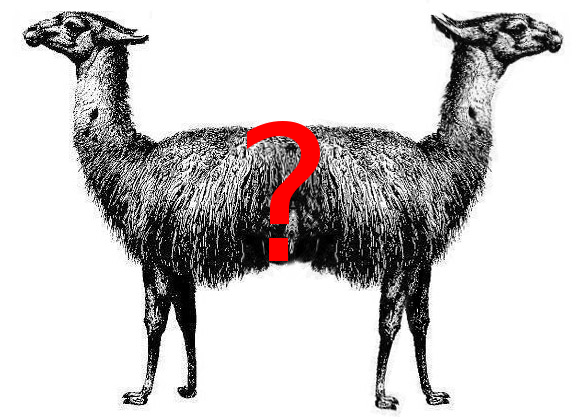
\includegraphics[width=0.75\textwidth]{pushmi-pullyu.png}
    \end{center}
  }
\end{frame}

\begin{frame}{Runtime Verification: \small A Summary}
  \begin{itemize}
    \item<1-> Only reasons about the current execution
    \item<1-> ``More decidable'' than static analysis
    \item<2-> But not incompatible with static analysis!
    \item<3-> Still a lot to be done in efficient and safe monitoring
      / error recovery
  \end{itemize}
\end{frame}

\begin{frame}{Questions?}
  \vspace{4.5cm}

  \footnotesize
  \textbf{Q:} What is the two-headed creature a few slides back?\\
  \textbf{A:} A pushmi-pullyu.

  \begin{quote}
    ``I notice,'' said the duck, ``that you only talk with one of your
    mouths. Can't the other head talk as well?''

    ``Oh, yes,'' said the pushmi--pullyu. ``But I keep the other mouth
    for eating---mostly. In that way I can talk while I am eating
    without being rude. Our people have always been very polite.''
  \end{quote}
\end{frame}

\end{document}